%\begin{sidewaysfigure}
%  \begin{center}
%  \includegraphics[width=0.8\textheight]{lhcb-detector-cross-section}
%  \caption[Cross-section view of \LHCb, cut in the non-bending $y$--$z$ plane]%
%    {Cross-section view of \LHCb, cut in the non-bending $y$--$z$ plane.}
%  \label{fig:LHCbCrossSection}
%  \end{center}
%\end{sidewaysfigure}



\chapter{Magnetic field simulation in ND280}
\label{chap:MagneticFieldSimulation}
ND280 is housed in the UA1 magnet which provides a 0.2 T magnetic field through the basket.  The purpose of this magnetic field is to aid particle identifcation in ND280's TPCs.  This magnetic field is accurately modelled in nd80mc by a constant 0.2 T magnetic field in the basket.  The ND280 analyses which are inputs to the oscillation analyses search for a TPC track matched to an FGD track so, in a first iteration of these analyses, the model is sufficient.
\newline
\newline
However, a significant part of the UA1 magnet is the iron magnetic flux return yoke which reroutes the magnetic field exiting the tracker so it can re-enter at the opposite side.  As a result, there is a significant magnetic field contained within the magnetic flux return yoke during operation.  This magnetic field in the flux return yoke is not modelled in nd280mc.  For the first iterations of the ND280 oscillation input analyses, this approximation was valid.  However, as the ND280 analyses become more mature, and non-tracker based analyses are started, this approximation is no longer valid.  So, the magnetic field model in the simulation needs revising. 

\section{Magnetic field model in the ND280 flux return}
\label{sec:MagneticFieldModel}
\begin{figure}
  \centering
  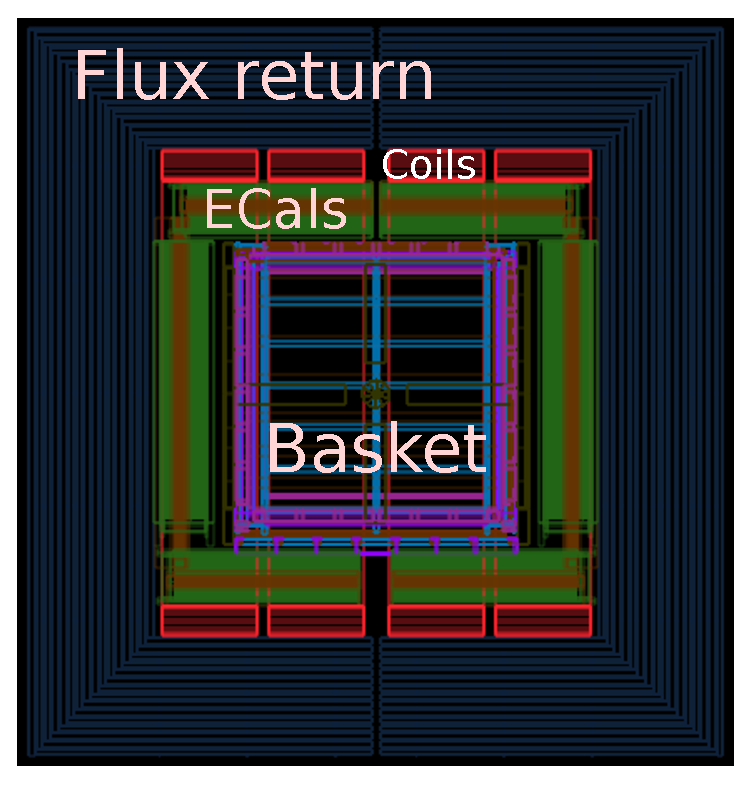
\includegraphics[width=9cm]{images/magnetic_field/ND280FluxReturn}
  \caption{Graphical display of the X--Y ND280 cross-section.}
  \label{fig:ND280FluxReturn}
\end{figure}
A simple model for the magnetic field in the flux return can be found by making two assumptions.  Firstly, the flux return yoke consists mostly of iron which has a much higher magnetic permeability than the air surrounding it.  So, it can be assumed that any magnetic flux passing through the ND280 basket is solely transported back around by the return yoke (no flux passes through the atmosphere in the pit).  It follows that
\begin{equation}
  \phi_{\textrm{b}} = \phi_{\textrm{r}},
  \label{eqn:BFluxConservation}
\end{equation}
where $\phi_{\textrm{b}}$ is the magnetic flux passing through the tracker and $\phi_{\textrm{r}}$ is the magnetic flux passing through the return yoke.  The second assumption regards the shape of the ND280 basket and flux return yoke.  The X--Y cross-section of ND280, as shown in Fig.~\ref{fig:ND280FluxReturn}, can be modelled as two distinct parts: the flux return yoke and everthing contained within.  It is clear from Fig.~\ref{fig:ND280FluxReturn} that both areas are retangular so the system can be modelled as a smaller rectange (the basket) contained within a larger rectange (the return yoke).  Using this assumption and Eq.~\ref{eqn:BFluxConservation}, the magnetic field strength passing through the return yoke, $B_{r}$, is
\begin{equation}
  B_{\textrm{r}} = \frac{B_{\textrm{b}}A_{\textrm{b}}}{A_{\textrm{r}} - A_{\textrm{b}}},
  \label{eqn:FluxReturnBField}
\end{equation}
where $B_{\textrm{b}}$ is the strength of the magnetic field passing through the basket, $A_{\textrm{b}}$ is the cross-sectional area of the basket region and $A_{\textrm{r}}$ is the cross-sectional area of the flux return yoke if the flux return yoke was not hollow.
\newline
\newline
\begin{figure}
  \centering
  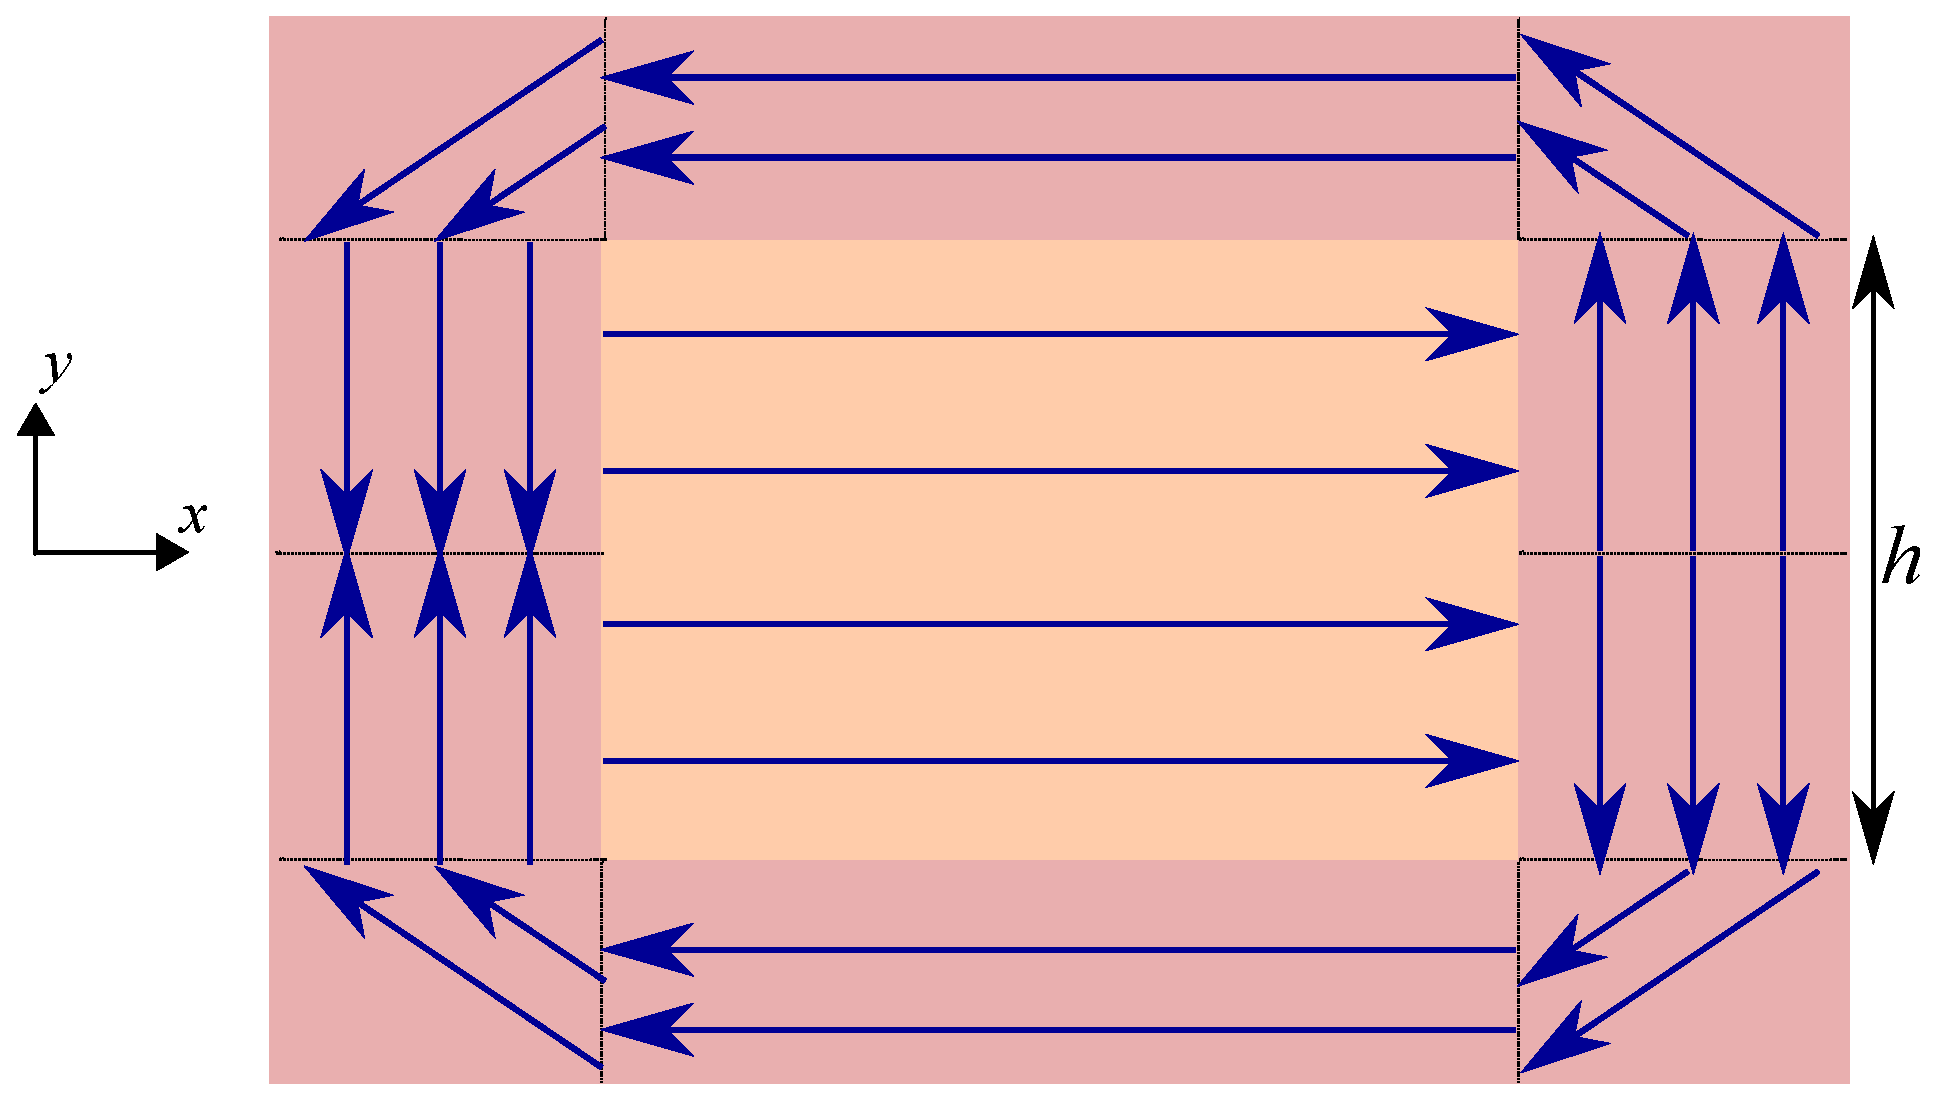
\includegraphics[width=9cm]{images/magnetic_field/BFieldDiagram}
  \caption{Simple model of the magnetic field in the basket and flux return region.  The flux return yoke has been separated into ten sections: four vertical B field sections, four corner B field sections and two horizontal B field sections.  The height of the basket region, $h$, is also shown.}
  \label{fig:BFieldDiagram}
\end{figure}
Eq.~\ref{eqn:FluxReturnBField} is sufficient to model the strength of the magnetic field in the flux return yoke.  However, Eq.~\ref{eqn:FluxReturnBField} conveys no information about the direction of the magnetic field but, the direction can be estimated by separating the flux return into ten sections as shown in Fig.~\ref{fig:BFieldDiagram}.  The sections are: four vertical sections where the magnetic field enters and exits the flux return region, two horizontal sections where the magnetic field in the flux return is anti-parallel to the magnetic field in the basket and four corner sections where the magnetic field transitions between the horizontal and vertical sections.  By defining the magnetic field in the basket to be parallel to the x-axis 
\begin{equation}
  \overrightarrow{B_{\textrm{b}}} = {B_{\textrm{b}}}\hat{\imath},
  \label{eqn:BasketBFieldVector}
\end{equation}
then it follows that the horizontal magnetic field in the flux return is
\begin{equation}
  \overrightarrow{B}^{\textrm{H}}_{\textrm{r}} = -{B_{\textrm{r}}}\hat{\imath}.
  \label{eqn:HorizontalReturnBFieldVector}
\end{equation}
The field model for the vertical section should take into account that the strength of the magnetic field is not constant, but increases in strength until it reaches the corner region.  The direction of the field depends on which vertical section is under consideration.  For the section where the magnetic field is exiting the tracker and moving upwards, the relevant vector is
\begin{equation}
  \overrightarrow{B}^{\textrm{V}}_{\textrm{r}} = \frac{y}{h/2}{B_{\textrm{r}}}\hat{\jmath},
  \label{eqn:VerticalReturnBFieldVector}
\end{equation}
where $h$ is the height of the ND280 basket and $y$ is the height where the magnetic field is being evaluated in the ND280 coordinate system.  In the corner regions, the magnetic field is defined to be straight, constant in strength and at 45$^\circ$ to the horizontal and vertical sections.  As with the vertical section, the magnetic field direction is dependent on which corner section is being considered.  For the corner section where the magnetic field is exiting the tracker and travelling vertically upwards (as defined in Eq.~\ref{eqn:VerticalReturnBFieldVector}), the vector is
\begin{equation}
  \overrightarrow{B}^{\textrm{C}}_{\textrm{r}} = \frac{B_{\textrm{r}}}{\sqrt{2}}(\hat{\jmath} - \hat{\imath}).
  \label{eqn:CornerReturnBFieldVector}
\end{equation}
The magnetic field in the other corner sections are then 45$^\circ$ rotations of Eq.~\ref{eqn:CornerReturnBFieldVector}.
\newline
\newline
This simple model of the magnetic field in the flux return has now been implemented in nd280mc.  Thus, any simulated charged-particles trajctory in the region surrounding the ECals (like muons entering from the pit region) will be altered by the new field.

\section{Effect of magnetic field on the ECal}
\label{sec:MagneticFieldEffect}
Better data/MC
